\chapter{专业知识}

\section{原码, 反码, 补码}
\begin{note}
本节系转载。转载经过了不改变原意的格式修改,并且删去了原文最后一部分《原码,反码,补码 再深入》。

作者:\href{http://www.cnblogs.com/zhangziqiu/}{张子秋}

出处:\url{https://www.cnblogs.com/zhangziqiu/archive/2011/03/30/computercode.html}

本小节版权归作者和博客园共有,欢迎转载,但未经作者同意必须保留此段声明,且在文章页面明显位置给出原文连接,否则保留追究法律责任的权利。
\end{note}

在学习原码,反码和补码之前,需要先了解机器数和真值的概念。

\paragraph*{机器数}一个数在计算机中的二进制表示形式,叫做这个数的机器数。机器数是带符号的,在计算机用一个数的最高位存放符号,正数为0,负数为1。比如,十进制中的数$+3$,计算机字长为8位,转换成二进制就是00000011。如果是$-3$,就是10000011。那么,这里的00000011和10000011就是机器数。

\paragraph*{真值}\label{sec6}
因为第一位是符号位,所以机器数的形式值就不等于真正的数值。例如上面的有符号数10000011,其最高位1代表负,其真正数值是$-3$而不是形式值131(10000011转换成十进制等于131)。所以,为区别起见,将带符号位的机器数对应的真正数值称为机器数的真值。
\begin{example}
$00000001\textnormal{的真值}=+0000001=+1$,$10000001\textnormal{的真值} = -0000001= -1$。
\end{example}

在探求为何机器要使用补码之前,让我们先了解原码,反码和补码的概念。对于一个数,计算机要使用一定的编码方式进行存储。原码,反码,补码是机器存储一个具体数字的编码方式。

\paragraph*{原码}
原码就是符号位加上真值的绝对值,即用第一位表示符号,其余位表示值。比如如果是8位二进制:
$$\begin{aligned}[]
[+1]_{\textrm{原}}=00000001\\
[-1]_{\textrm{原}}=10000001
\end{aligned}$$
第一位是符号位。因为第一位是符号位,所以8位二进制数的取值范围就是:$[11111111,01111111]$,即$[-127,127]$。原码是人脑最容易理解和计算的表示方式。

\paragraph*{反码}
反码的表示方法是:
\begin{itemize}
\item 正数的反码是其本身。
\item 负数的反码是在其原码的基础上,符号位不变,其余各个位取反。
\end{itemize}
$$\begin{aligned}[]
[+1]=[00000001]_{\textrm{原}}=[00000001]_{\textrm{反}}\\
[-1]=[10000001]_{\textrm{原}}=[11111110]_{\textrm{反}}
\end{aligned}$$
可见如果一个反码表示的是负数,人脑无法直观的看出来它的数值。通常要将其转换成原码再计算。

\paragraph*{补码}
补码的表示方法是:
\begin{itemize}
\item 正数的补码就是其本身。
\item 负数的补码是在其原码的基础上,符号位不变,其余各位取反,最后$+1$。(即在反码的基础上$+1$)
\end{itemize}
$$\begin{aligned}[]
[+1]=[00000001]_{\textrm{原}}=[00000001]_{\textrm{反}}=[00000001]_{\textrm{补}}\\
[-1]=[10000001]_{\textrm{原}}=[11111110]_{\textrm{反}}=[11111111]_{\textrm{补}}
\end{aligned}$$
对于负数,补码表示方式也是人脑无法直观看出其数值的。通常也需要转换成原码在计算其数值。

\paragraph*{为何要使用原码,反码和补码}
在开始深入学习前,我的学习建议是先“死记硬背”上面的原码,反码和补码的表示方式以及计算方法。现在我们知道了计算机可以有三种编码方式表示一个数。对于正数因为三种编码方式的结果都相同:
$$[+1]=[00000001]_{\textrm{原}}=[00000001]_{\textrm{反}}=[00000001]_{\textrm{补}}$$
所以不需要过多解释。但是对于负数:
$$[-1]=[10000001]_{\textrm{原}}=[11111110]_{\textrm{反}}=[11111111]_{\textrm{补}}$$
可见原码,反码和补码是完全不同的。既然原码才是被人脑直接识别并用于计算表示方式,为何还会有反码和补码呢?

首先,因为人脑可以知道第一位是符号位,在计算的时候我们会根据符号位,选择对真值区域的加减(\hyperref[sec6]{真值的概念})。但是对于计算机,加减乘数已经是最基础的运算,要设计的尽量简单。计算机辨别“符号位”显然会让计算机的基础电路设计变得十分复杂!于是人们想出了将符号位也参与运算的方法。我们知道,根据运算法则减去一个正数等于加上一个负数,即:$1-1=1+(-1)=0$,所以机器可以只有加法而没有减法,这样计算机运算的设计就更简单了。

于是人们开始探索将符号位参与运算,并且只保留加法的方法。首先来看原码:

计算十进制的表达式:$1-1=0$
$$1-1=1+(-1)=[00000001]_{\textrm{原}}+[10000001]_{\textrm{原}}=[10000010]_{\textrm{原}}=-2$$
如果用原码表示,让符号位也参与计算,显然对于减法来说,结果是不正确的。这也就是为何计算机内部不使用原码表示一个数。为了解决原码做减法的问题,出现了反码:

计算十进制的表达式:$1-1=0$
\[\begin{split}
1-1&=1+(-1)=[00000001]_{\textrm{原}}+[10000001]_{\textrm{原}}=[00000001]_{\textrm{反}}+[11111110]_{\textrm{反}}\\
&=[11111111]_{\textrm{反}}=[10000000]_{\textrm{原}}=-0
\end{split}\]
发现用反码计算减法,结果的真值部分是正确的。而唯一的问题其实就出现在“0”这个特殊的数值上。虽然人们理解上$+0$和$-0$是一样的,但是0带符号是没有任何意义的。而且会有$[00000000]_{\textrm{原}}$和$[10000000]_{\textrm{原}}$两个编码表示0。

于是补码的出现,解决了0的符号以及两个编码的问题:
\[\begin{split}
1-1&=1+(-1)=[00000001]_{\textrm{原}}+[10000001]_{\textrm{原}}=[00000001]_{\textrm{补}}+[11111111]_{\textrm{补}}\\
&=[00000000]_{\textrm{补}}=[00000000]_{\textrm{原}}
\end{split}\]
这样0用$[00000000]$表示, 而以前出现问题的$-0$则不存在了。而且可以用$[10000000]$表示$-128$:
$$(-1)+(-127)=[10000001]_{\textrm{原}}+[11111111]_{\textrm{原}}=[11111111]_{\textrm{补}}+[10000001]_{\textrm{补}}=[10000000]_{\textrm{补}}$$
$-1-127$的结果应该是$-128$,在用补码运算的结果中,$[1000 0000]_{\textrm{补}}$就是$-128$。但是注意因为实际上是使用以前的$-0$的补码来表示$-128$,所以$-128$并没有原码和反码表示。(对$-128$的补码表示$[10000000]_{\textrm{补}}$算出来的原码是$[0000 0000]_{\textrm{原}}$, 这是不正确的)

使用补码,不仅仅修复了0的符号以及存在两个编码的问题,而且还能够多表示一个最低数。这就是为什么8位二进制,使用原码或反码表示的范围为$[-127,+127]$,而使用补码表示的范围为$[-128,127]$。

因为机器使用补码,所以对于编程中常用到的32位int类型,可以表示范围是:$[-2^{31},2^{31}-1]$ 因为第一位表示的是符号位,而使用补码表示时又可以多保存一个最小值。

\section{浮点数}
\begin{note}
本节系摘编。

版权声明:本小节为博主原创文章,遵循\href{http://creativecommons.org/licenses/by-sa/4.0/}{CC 4.0 BY-SA}版权协议,转载请附上原文出处链接和本声明。

原文链接:\url{https://blog.csdn.net/shuzfan/article/details/53814424}
\end{note}

\paragraph*{浮点数表示}
浮点数是一种\textbf{公式化}的表达方式,用来近似表示实数,并且可以在表达范围和表示精度之间进行权衡(因此被称为浮点数)。

浮点数通常被表示为:
$$N=M\times R^E$$
比如:$12.345=1.2345\times 10^1$。

其中,$M$(Mantissa)被称为浮点数的\textbf{尾数},$R$(Radix)被称为阶码的\textbf{基数},$E$(Exponent)被称为阶的\textbf{阶码}。计算机中一般规定$R$为2、8或16,是一个确定的常数,不需要在浮点数中明确表示出来。

因此,在已知标准下,要表示浮点数,

一是要给出尾数M的值,通常用定点小数形式表示,它决定了浮点数的表示精度,即可以给出的有效数字的位数。

二是要给出阶码,通常用定点整数形式表示,它指出的是小数点在数据中的位置,决定了浮点数的表示范围。因此,在计算机中,浮点数通常被表示成如\autoref{fig5}所示格式。(假定为32位浮点数,基为2,其中最高位为符号位)

\begin{figure}[!ht]
\centering
\includegraphics[width=\textwidth]{images/358.png}
\caption{}\label{fig5}
\end{figure}

\paragraph*{浮点数的规格化表示}
按照上面的指数表示方法,一个浮点数会有不同的表示:
$$0.3\times 10^0;\quad 0.03\times 10^1;\quad 0.003\times10^2;\quad 0.0003\times 10^3$$
\textbf{为了提高数据的表示精度同时保证数据表示的唯一性,需要对浮点数做规格化处理。}

\textbf{在计算机内,对非0值的浮点数,要求尾数的绝对值必须大于基数的倒数,即$|M|\ge\frac{1}{R}$。}

即要求尾数域的最高有效位应为1,称满足这种表示要求的浮点数为规格化表示:把不满足这一表示要求的尾数,变成满足这一要求的尾数的操作过程,叫作浮点数的规格化处理,通过尾数移位和修改阶码实现。

比如,二进制原码的规格化数的表现形式:(0正1负)
\begin{itemize}
\item 正数 0.1xxxxxx
\item 负数 1.1xxxxxx
\end{itemize}

\textbf{注意,尾数的最高位始终是1,因此我们完全可以省略掉该位。}

至此,我们引入IEEE754标准,该标准约束了浮点数的大部分使用设置:
\begin{itemize}
\item \textbf{尾数用原码,且隐藏尾数最高位。}

原码非0值浮点数的尾数数值最高位必定为 1,因此可以忽略掉该位,这样用同样多的位数就能多存一位二进制数,有利于提高数据表示精度,称这种处理方案使用了隐藏位技术。当然,在取回这样的浮点数到运算器执行运算时,必须先恢复该隐藏位。
\item \textbf{阶码使用“移码”,基固定为2}

如\autoref{fig6}的32bit浮点数和64bit浮点数,从最高位依次是符号位、阶码和尾数 
\begin{figure}[!ht]
\centering
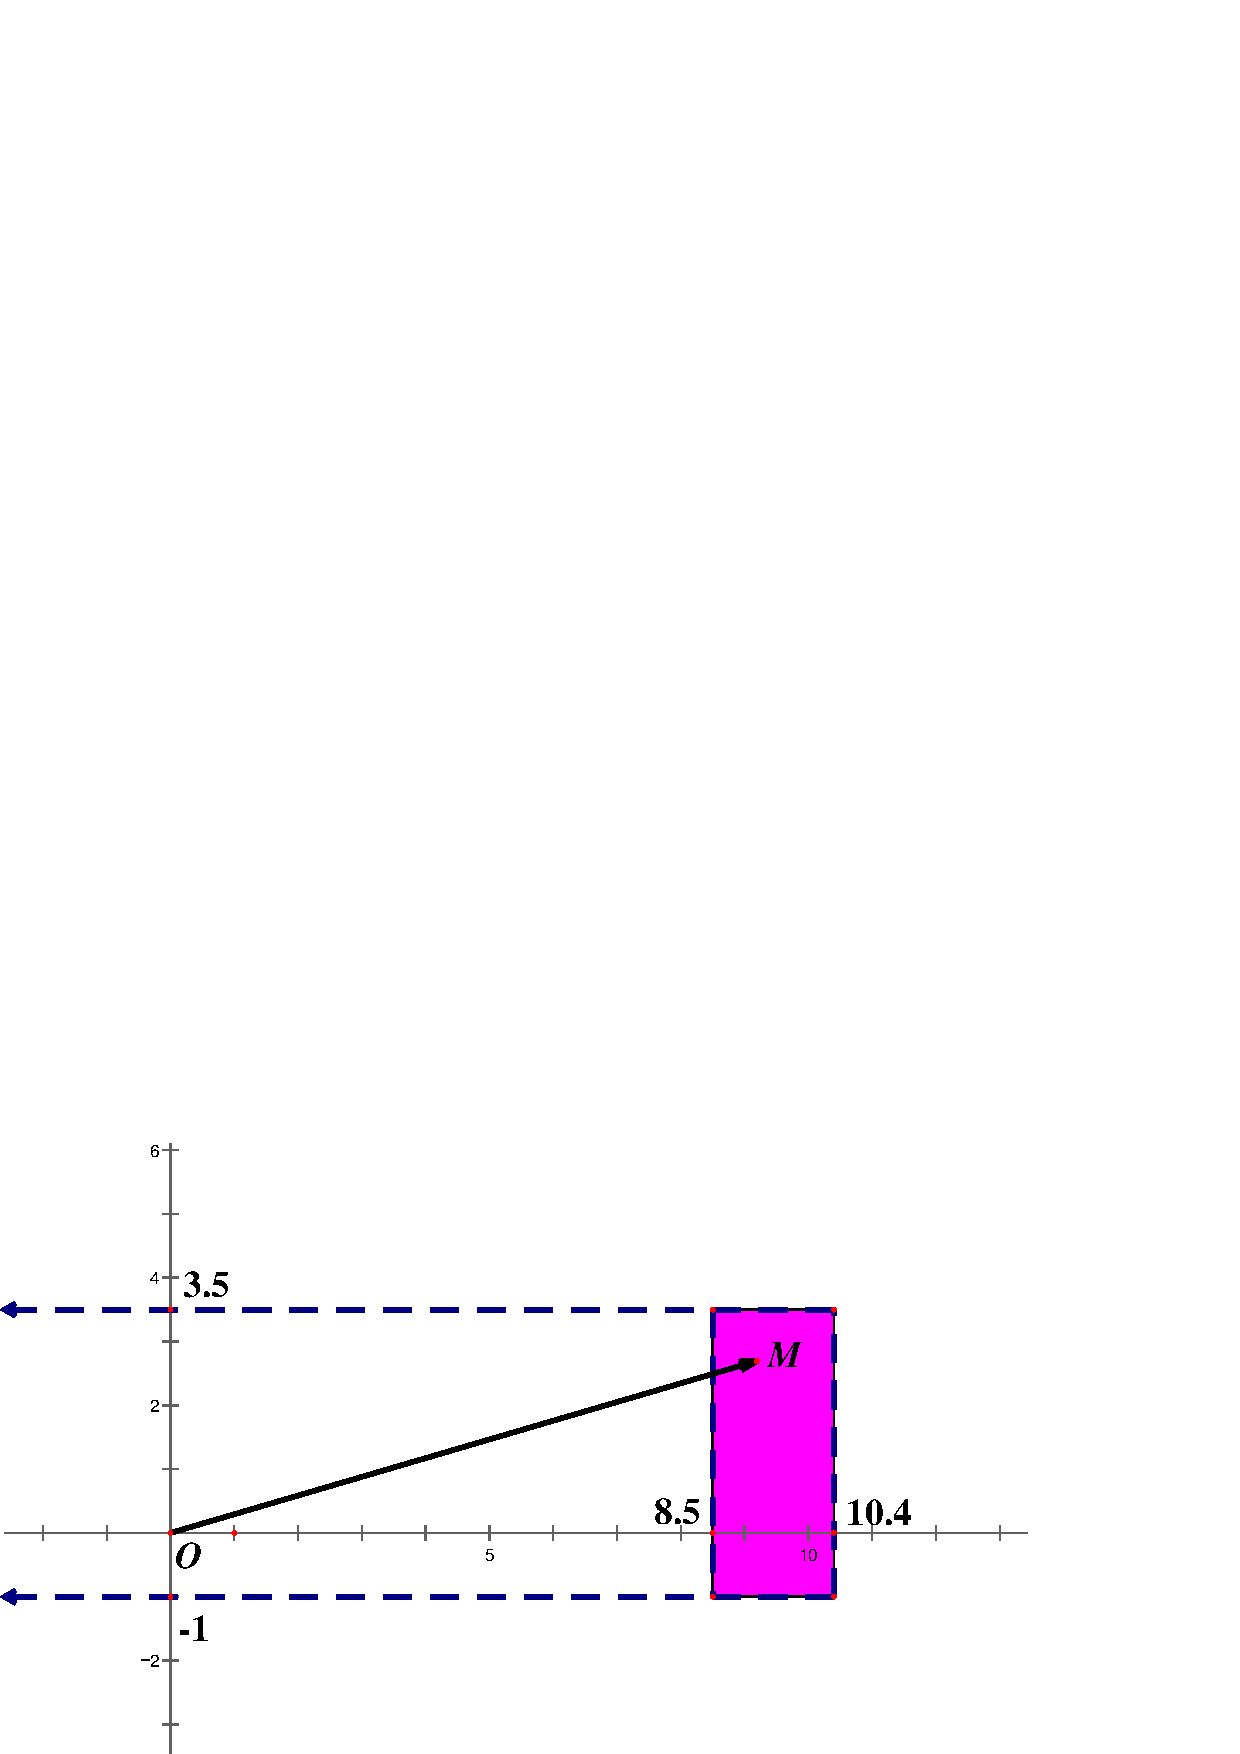
\includegraphics[width=\textwidth]{images/1.jpg}
\caption{}\label{fig6}
\end{figure}
于是,一个规格化的32位浮点数x的真值为:
$$x=(-1)^S\times(1.M)\times 2^{E-127}$$
一个规格化的64位浮点数x的真值为:
$$x=(-1)^S\times(1.M)\times 2^{E-1023}$$
\end{itemize}

下面举一个32位单精度浮点数-3.75表示的例子帮助理解:
\begin{itemize}
\item 首先转化为2进制表示
$$?3.75=?(2+1+1/2+1/4)=?1.111\times 2^1$$
\item 整理符号位并进行规格化表示
$$?1.111\times 2^1=(?1)^{(1)}\times (1+0.1110\,0000\,0000\,0000\,0000\,000)\times 2^1$$
\item 进行阶码的移码处理 
$$(?1)^{(1)}\times (1+0.1110\,0000\,0000\,0000\,0000\,000)\times 2^1=(?1)^{(1)}\times (1+0.1110\,0000\,0000\,0000\,0000\,000)\times 2^{128?127}$$
\end{itemize}
于是,符号位$S=1$,尾数$M$为$1110\,0000\,0000\,0000\,0000\,000$,阶码$E$为$128_{10}=1000\,0000_2$,则最终的32位单精度浮点数为
$$1\,1000\,0000\,1110\,0000\,0000\,0000\,0000\,000$$

\section{BCD码与二进制码的转换}
\subsection{BCD码简介}
\begin{note}
本节系摘编。

版权声明:本小节为博主原创文章,遵循\href{http://creativecommons.org/licenses/by-sa/4.0/}{CC 4.0 BY-SA}版权协议,转载请附上原文出处链接和本声明。

原文链接:\url{https://blog.csdn.net/qq_33750826/article/details/53004685}
\end{note}

Binary-Coded Decimal,简称BCD,称BCD码或二-十进制代码,亦称二进码十进数。是一种二进制的数字编码形式,用二进制编码的十进制代码。这种编码形式利用了四个位元来储存一个十进制的数码,使二进制和十进制之间的转换得以快捷的进行。这种编码技巧,最常用于会计系统的设计里,因为会计制度经常需要对很长的数字串作准确的计算。相对于一般的浮点式记数法,采用BCD码,既可保存数值的精确度,又可免却使电脑作浮点运算时所耗费的时间。此外,对于其他需要高精确度的计算,BCD编码亦很常用。

由于十进制数共有0、1、2、……、9十个数码,因此,至少需要4位二进制码来表示1位十进制数。在使用BCD编码时一定要注意其有效的编码仅十个,即:0000~1001.四位二进制数的其余六个编码1010,1011,1100,1101,1110,1111不是有效编码。常见BCD编码有8421BCD码,2421BCD码,余3码,对应编码表如\autoref{tab3}。\textbf{本文档中使用8421码}。
\begin{table}[!ht]
\centering
\begin{tabular}{|c|c|c|c|}
\hline
十进制数&8421码&2421码&余3码\\\hline
0&0000&0000&0011\\\hline
1&0001&0001&0100\\\hline
2&0010&0010&0101\\\hline
3&0011&0011&0110\\\hline
4&0100&0100&0111\\\hline
5&0101&1011&1000\\\hline
6&0110&1100&1001\\\hline
7&0111&1101&1010\\\hline
8&1000&1110&1011\\\hline
9&1001&1111&1100\\\hline
\end{tabular}
\caption{常见的BCD编码。通常开发使用8421,8421对于新手能一看就懂。}\label{tab3}
\end{table}

\subsection{BCD码转二进制}\label{sec30}
BCD码是我们用来表示十进制数的方式,BCD转二进制的算法也就是十进制转二进制的算法。这里我们介绍短除法,该算法是高中课程的内容。

短除法将一个数反复除以2直到商为0,取余数倒序为二进制结果。
\begin{example}
将19转为二进制。
\begin{align*}
19&\div2=9\cdots1\\
9&\div2=4\cdots1\\
4&\div2=2\cdots0\\
2&\div2=1\cdots0\\
1&\div2=0\cdots1
\end{align*}
余数的倒序10011即为19的二进制表示。
\end{example}

对于BCD而言,我们可以通过一些简单的运算来代替除以2,取商和余数的运算。除法是复杂运算,所以用简单运算代替除法的收益很高。为了理解这种方法,我们先来回顾一下小学学过的长除法。
\begin{example}
用BCD码长除法计算123456789除以2的商和余数。
$$\begin{array}{|r|rrrrrrrrr|}
\hline
\textnormal{商}&0000&0110&0001&0111&0010&1000&0011&1001&0100\\\hline
\textnormal{被除数}&0001&0010&0011&0100&0101&0110&0111&1000&1001\\
&0000&&&&&&&&\\\cline{2-2}
&   1&0010&&&&&&&\\
&   1&0010&&&&&&&\\\cline{2-3}
&    &   0&0011&&&&&&\\
&	&    &0010&&&&&&\\\cline{3-4}
&	&    &   1&0100&&&&&\\
&	&    &   1&0100&&&&&\\\cline{4-5}
&	&    &    &   0&0101&&&&\\
&	&    &    &    &0100&&&&\\\cline{5-6}
&	&    &    &    &   1&0110&&&\\
 &   &    &    &    &   1&0110&&&\\\cline{6-7}
	&&	 &	  &	   &	&   0&0111&&\\
	&&	 &	  &	   &	&   0&0110&&\\\cline{7-8}
	&&	 &	  &	   &	&	 &	 1&1000&\\
	&&	 &	  &	   &	&	 &	 1&1000&\\\cline{8-9}
	&&	 &	  &	   &	&	 &	  &	  0&1001\\
	&&	 &	  &	   &	&	 &	  &	  0&1000\\\hline
\textnormal{余数}&&	 &	  &	   &	&	 &	  &	   &   1\\\hline
\end{array}$$
\end{example}

从除数为2的长除法过程中(不仅包括上面的例子),我们发现了如下规律:
\begin{enumerate}
\item 某一个十进制位的BCD码的最后一位就是除到这一位后留下的余数。
\item 商的某一个十进制位取值取决于被除数对应十进制位BCD码的前三位和前一个十进制位BCD码的后一位,具体见\autoref{tab5}。
\end{enumerate}

\begin{table}[!ht]
\centering
\begin{tabular}{|r|l|c|r|}
\hline
\thead{被除数\\ 前一个\\ 十进制位\\ BCD码}&\thead{被除数\\ 对应\\ 十进制位\\ BCD码}&\thead{商}&解释\\\hline
XXX0&000X&0000&$0,1\div 2=0$\\\hline
XXX0&001X&0001&$2,3\div 2=1$\\\hline
XXX0&010X&0010&$4,5\div 2=2$\\\hline
XXX0&011X&0011&$6,7\div 2=3$\\\hline
XXX0&100X&0100&$8,9\div 2=4$\\\hline
XXX1&000X&0101&$10,11\div 2=5$\\\hline
XXX1&001X&0110&$12,13\div 2=6$\\\hline
XXX1&010X&0111&$14,15\div 2=7$\\\hline
XXX1&011X&1000&$16,17\div 2=8$\\\hline
XXX1&100X&1001&$18,19\div 2=9$\\\hline
\end{tabular}
\caption{X表示0或1}\label{tab5}
\end{table}

在这个除法中,商的每个十进制的4位BCD码由被除数BCD码中错位的4位唯一确定,其对应关系已经由\autoref{tab5}给出。而余数就是被除数BCD码的最后一位。至此,我们已经得到了不通过除法运算直接得到商和余数的方法。反复执行该方法,就可以将BCD转换为二进制。

\begin{example}\label{exa2}
将十进制数123转为二进制。
\begin{enumerate}
\item 写下123的BCD码1 0010 0011;
\item 取出最后一位1作为第一个余数,将剩下8位从右向左每4位分一组:1001 0001;查\autoref{tab5}得到商为0110 0001($123\div 2=61\cdots 1$);
\item 取出最后一位1作为第二个余数,将剩下数字从右向左每4位分一组:0011 0000;查\autoref{tab5}得到商为0011 0000($61\div 2=30\cdots 1$);
\item 取出最后一位0作为第三个余数,将剩下数字从右向左每4位分一组:0001 1000;查\autoref{tab5}得到商为0001 0101($30\div 2=15\cdots 0$);
\item 取出最后一位1作为第四个余数,将剩下数字从右向左每4位分一组:1010;查\autoref{tab5}得到商为0111($15\div 2=7\cdots 1$);
\item 取出最后一位1作为第五个余数,将剩下数字从右向左每4位分一组:0011;查\autoref{tab5}得到商为0011($7\div 2=3\cdots 1$);
\item 取出最后一位1作为第六个余数,将剩下数字从右向左每4位分一组:0001;查\autoref{tab5}得到商为0001($3\div 2=1\cdots 1$);
\item 取出最后一位1作为第七个余数,将剩下数字从右向左每4位分一组:0000;查\autoref{tab5}得到商为0000($1\div 2=0\cdots 1$);
\item 将所有余数倒序列出,1111011就是123的二进制表示。
\end{enumerate}
\end{example}

以上每一步中,执行取余、分组、查表三步,我们把这三步合并,用竖式简单地表达出来:
\begin{example}\label{exa1}
将BCD码100100011转为二进制。
\begin{center}
\begin{tabular}{|ccccccccc|}
\hline
1&0&0&1&\multicolumn{1}{|c}{0}&0&0&1&\multicolumn{1}{|c|}{1}\\\hline
0&1&1&\multicolumn{1}{|c}{0}&0&0&0&\multicolumn{1}{|c}{1}&1\\\hline
0&1&\multicolumn{1}{|c}{1}&0&0&0&\multicolumn{1}{|c}{0}&1&1\\\hline
0&\multicolumn{1}{|c}{1}&0&1&0&\multicolumn{1}{|c}{1}&0&1&1\\\hline
0&0&1&1&\multicolumn{1}{|c}{1}&1&0&1&1\\\hline
0&0&1&\multicolumn{1}{|c}{1}&1&1&0&1&1\\\hline
0&0&\multicolumn{1}{|c}{1}&1&1&1&0&1&1\\\hline
\end{tabular}
\end{center}
\end{example}

\subsection{二进制转BCD码}\label{sec31}
回顾\autoref{exa1}中的算法。每一步中,进行分离最后一位、分组、查表三个操作,最终从第一行的BCD码推到了最后一行的二进制。每一步都是由\autoref{tab5}唯一确定的,所以可以作为一个可靠的算法。反过来想,如果先知道了最后一行的二进制,是否可以反推到第一行的BCD码呢?我们来试试。
\begin{example}
将二进制1111011转为BCD码。尝试将\autoref{exa2}中的步骤反向。
\begin{enumerate}
\item 二进制数是1111011。
\item 取0作为商,从右向左每4位分一组:0000;查\autoref{tab5}得到被除数为0000X,用二进制数的第一位代替X并重新分组得到被除数为0001($1\div 2=0\cdots 1$);
\item 取上一步的被除数0001作为商;查\autoref{tab5}得到被除数为0001 X;用二进制数的第二位代替X并重新分组得到被除数为0011($3\div 2=1\cdots 1$);
\item 取上一步的被除数0011作为商;查\autoref{tab5}得到被除数为0011 X;用二进制数的第三位代替X并重新分组得到被除数为0111($7\div 2=3\cdots 1$);
\item 取上一步的被除数0111作为商;查\autoref{tab5}得到被除数为1010 X;用二进制数的第四位代替X并重新分组得到被除数为0001 0101($15\div 2=7\cdots 1$);
\item 取上一步的被除数0001 0101作为商;查\autoref{tab5}得到被除数为0001 1000 X;用二进制数的第五位代替X并重新分组得到被除数为0011 0000($30\div 2=15\cdots 0$);
\item 取上一步的被除数0011 0000作为商;查\autoref{tab5}得到被除数为0011 0000 X;用二进制数的第六位代替X并重新分组得到被除数为0110 0001($61\div 2=30\cdots 1$);
\item 取上一步的被除数0110 0001作为商;查\autoref{tab5}得到被除数为1001 0001 X;用二进制数的第七位代替X并重新分组得到被除数为0001 0010 0011($123\div 2=61\cdots 1$);
\item 所求的BCD码为1 0010 0011。
\end{enumerate}
上面的步骤写成竖式就是
\begin{center}
\begin{tabular}{|ccccccccc|}
\hline
0&0&1&\multicolumn{1}{|c}{1}&1&1&0&1&1\\\hline
0&0&1&1&\multicolumn{1}{|c}{1}&1&0&1&1\\\hline
0&0&1&1&1&\multicolumn{1}{|c}{1}&0&1&1\\\hline
0&1&\multicolumn{1}{|c}{0}&1&0&1&\multicolumn{1}{|c}{0}&1&1\\\hline
0&1&1&\multicolumn{1}{|c}{0}&0&0&0&\multicolumn{1}{|c}{1}&1\\\hline
0&1&1&0&\multicolumn{1}{|c}{0}&0&0&1&\multicolumn{1}{|c|}{1}\\\hline
1&\multicolumn{1}{|c}{0}&0&1&0&\multicolumn{1}{|c}{0}&0&1&1\\\hline
\end{tabular}
\end{center}
\end{example}

\section{$\mathbb{Z}_2$上的线性代数}
\subsection{域$\mathbb{Z}_2$简介}
把整数分成奇数和偶数,则有如下运算规律:
\begin{center}
\begin{tabular}{|c|cc|}
\hline
$+$&偶&奇\\\hline
偶&偶&奇\\
奇&奇&偶\\\hline
\end{tabular}
\begin{tabular}{|c|cc|}
\hline
$\times$&偶&奇\\\hline
偶&偶&偶\\
奇&偶&奇\\\hline
\end{tabular}
\end{center}

$\mathbb{Z}_2=\{0,1\}$表示整数除2所得余数的集合,则0代表偶数,1代表奇数,0和1之间的加法和乘法运算遵守上述奇偶的运算规律,即
\begin{center}
\begin{tabular}{|c|cc|}
\hline
$+$&0&1\\\hline
0&0&1\\
1&1&0\\\hline
\end{tabular}
\begin{tabular}{|c|cc|}
\hline
$\times$&0&1\\\hline
0&0&0\\
1&0&1\\\hline
\end{tabular}
\end{center}

另外,定义除法为乘法的逆运算,即$0\div 1=0$、$1\div 1=1$,除数不能为0。定义减法为加法的逆运算,由于$\mathbb{Z}_2$的特殊性,减法和加法的运算规则完全一样。

如果将0和1又看作逻辑中的真和假,则加法对应的是异或,乘法对应的是与,所以可以用$\mathbb{Z}_2$上的运算来描述逻辑。

\subsection{向量与线性组合}